\documentclass[main.tex]{subfiles}
\begin{document}

\subsection{Digitized Waveform Neutron Tagging}

\subsubsection{Pulse shape discrimination: Charge comparisson}
Just like with the analog setup the charge integrals were used to perform pulse shape discrimination. The resulting PSD heatmap is shown figure \ref{fig:psd_d}. Since a lower amplitude threshold was applied to the digital setup we find a lot of low energy gamma rays in the gamma band. The 2.23 $MeV_{ee}$ and 4.44 $MeV_{ee}$ compton edges are also clearly distinguishable. 

As with the analog setup longgate and shortgate offsets can be used to linearize the seperation between the bands. Here each shortgate sample point has been offset by 4.79 mV while each longgate sample has been offset by 0.24 mV. At lower energies the bands intersect, but above 1.5 MeV they are clearly separated.

\begin{figure}[ht]
    \centering
        \includegraphics{DigitalResults/psd.pdf}
        \caption{Pulse shape discrimination spectrum produced with the charge comparisson method.}
        \label{fig:psd_d}
\end{figure}

\subsubsection{Pulse shape discrimination: Convolutional neural network}
The convolutional neural network described in \ref{sec:cnn} was applied to the digitized waveforms. Since the activation function of the output node is the logistic function the value is bounded between zero and one. The resulting pulse shape discrimination spectrum is shown in figure \ref{fig:cnn_E} as a function of deposited energy. Like for the charge comparisson method the upper distribution is neutrons and the lower distribution consists of gamma rays. The bands a much better separated than by the charge comparisson method although the still is some slight overlap at low energies. Again the 2.23 and 4.44 $MeV_{ee}$ Compton edges are clearly visible in the gamma band. 

\begin{figure}[ht]
    \centering
        \includegraphics{DigitalResults/CNNpsd.pdf}
        \caption{Pulse shape discrimination spectrum produced with a convolutional neural network.}
    \label{fig:cnn_E} 
\end{figure}

\clearpage
\subsubsection{Time of flight spectrum}
The time of flight spectrum acquired in the 1 hour of data taking is shown in figure \ref{fig:tof_d}. The gamma and netron peaks are indicated with arrows. The gamma peak is not entirely narrow as one might expect seeing as they all travel at the speed of light. As for the analog setup part of the reason is that each photon may have a longer or shorter flightpath depending on its point of production in the source and the point at which it interacts in the detector. Furthermore, the time resolution is limited by is limited by the digitization process. The CFD algorithm looks for where the pulse crosses 30\% of maximum amplitude, but the determination of the maximum amplitude is limited by the resolution and sampling rate of the digitizer.

The flight times in the neutron peak, marked with dotted red lines, has been used to generate the energy spectrum shown in the upper right insert of figure \ref{fig:tof_d}. The spectrum goes to lower energies than what we see for the analog setup in figure \ref{fig:tof_a}, this may be because the digital setup has a lower amplitude threshold than the analog setup, allowing slower neutrons to be recorded.
\begin{figure}[ht]
    \centering
        \includegraphics{DigitalResults/tof.pdf}
        \caption{The time of flight spectrum of the PuBe source produced by the digital setup.}
    \label{fig:tof_d} 
\end{figure}

In order to test the two pulse shape discrimination algorithms one can plot their pulse shape parameters against time of flight. This is shown in figure \ref{fig:tof_cc_tof_cnn}. Figure \ref{fig:tof_digi_cc} shows the narrow gamma distribution and the wider neutron distribution as separated by the charge comparisson method. It is apparent that the two distributons overlap somewhat in pulse shape. It is of note that the neutron and gamma background forms two slightly separated bands.  In figure \ref{fig:tof_digi_cnn} it can be seen that the CNN method provides a better separation, although it still appears that gamma and neutron distributions overlap slightly near prediction value 0.5. The distribution of random coincidence events clearly separate into a gamma ray band below the cut and a neutron band above it.


\begin{figure}
    \centering
    \begin{subfigure}[ht]{\textwidth}
        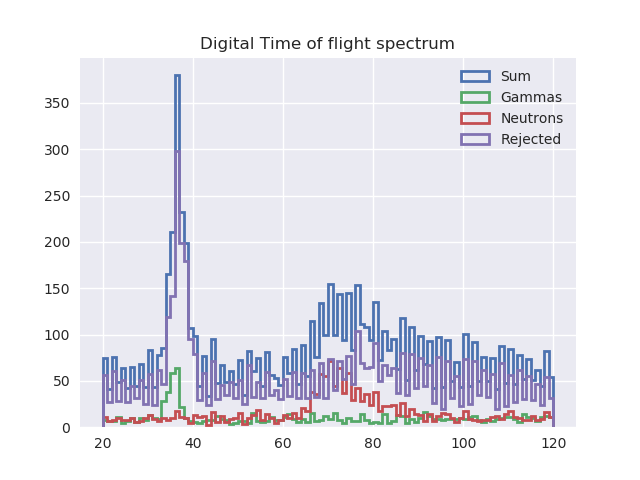
\includegraphics{DigitalResults/tof_psd.pdf}
        \caption{}
        \label{fig:tof_digi_cc}
    \end{subfigure}
	\begin{subfigure}[ht]{\textwidth}
        \includegraphics{DigitalResults/CNNtof_psd.pdf}
        \caption{}
        \label{fig:tof_digi_cnn}
    \end{subfigure}
    \caption{Heatmaps of of pulseshape discrimination parameters as functions of time of flight plotted with logarithmic z-axis.}
    \label{fig:tof_cc_tof_cnn}
\end{figure}

The heatmap shown in figure \ref{fig:tof_E_d} shows energy deposition in the NE213 detector as a function of time of flight. This spectrum can help us understand why the gamma spectrum is not entirely narrow. It seems that low energy gamma rays are a bit more spread out regarding time of flight. This could mean that the CFD algorithm has a harder time timestamping low charge pulses or that gamma rays traveling at an angle and hitting the the detector closer to the edge have a larger chance of scattering out of it without depositing all their energy. The neutron distribution clearly shows a relation between time of flight and deposited energy. In figure \ref{fig:tof_Edep_Eneutron_d} this relation is highlighted. There appears to be a roughly linear relation between maximum deposited energy and neutron kinetic energy. However, as for the analog setup a neutron may deposit all or only part of its energy, so for a given deposited energy we can only conclude the minimum amount of energy the neutron must have had.


\begin{figure}[ht]
    \centering
        \includegraphics{DigitalResults/tof_E.pdf}
        \caption{Time of flight plotted against energy deposition.}
    \label{fig:tof_E_d} 
\end{figure}

\begin{figure}[ht]
    \centering
        \includegraphics{DigitalResults/tof_Edep_Eneutron.pdf}
        \caption{Neutron energy as a function of deposited energy in the NE213 detector.}
    \label{fig:tof_Edep_Eneutron_d} 
\end{figure}




\end{document}